\subsubsection{\gls*{mca} transformacijos klasifikatoriaus tikslumo nustatymas}\label{sec:exp:4}

\gls{mca} klasifikatorius yra vienas iš standartinių klasifikatorių (šiuo atveju atsitiktinio miško \angl{random forest}), naudojantis pakeistos bazės požymius kaip įvestį. Šioje vietoje naudojamas klasifikatorius gali būti bet koks, tačiau turi būti suderinamas su \gls{mca} komponenčių kiekio reikalavimais \skyrius{sec:method:mca_comp_selection}. 

Kaip ir originalus klasifikatorius, šis negeba išskirti obfuskuotų programų, tad \ref{fig:exp4:confusion} pav. pateikiamoje klasifikavimo lentelėje rodomas prognozuojamos klasės ir visų tai klasei priklausančių duomenų santykis.
Eksperimento rezultatai (klasifikavimo metrikos) pateikiami \ref{tbl:exp4:metrics}-oje lentelėje.
\begin{figure}[h]
    \centering
    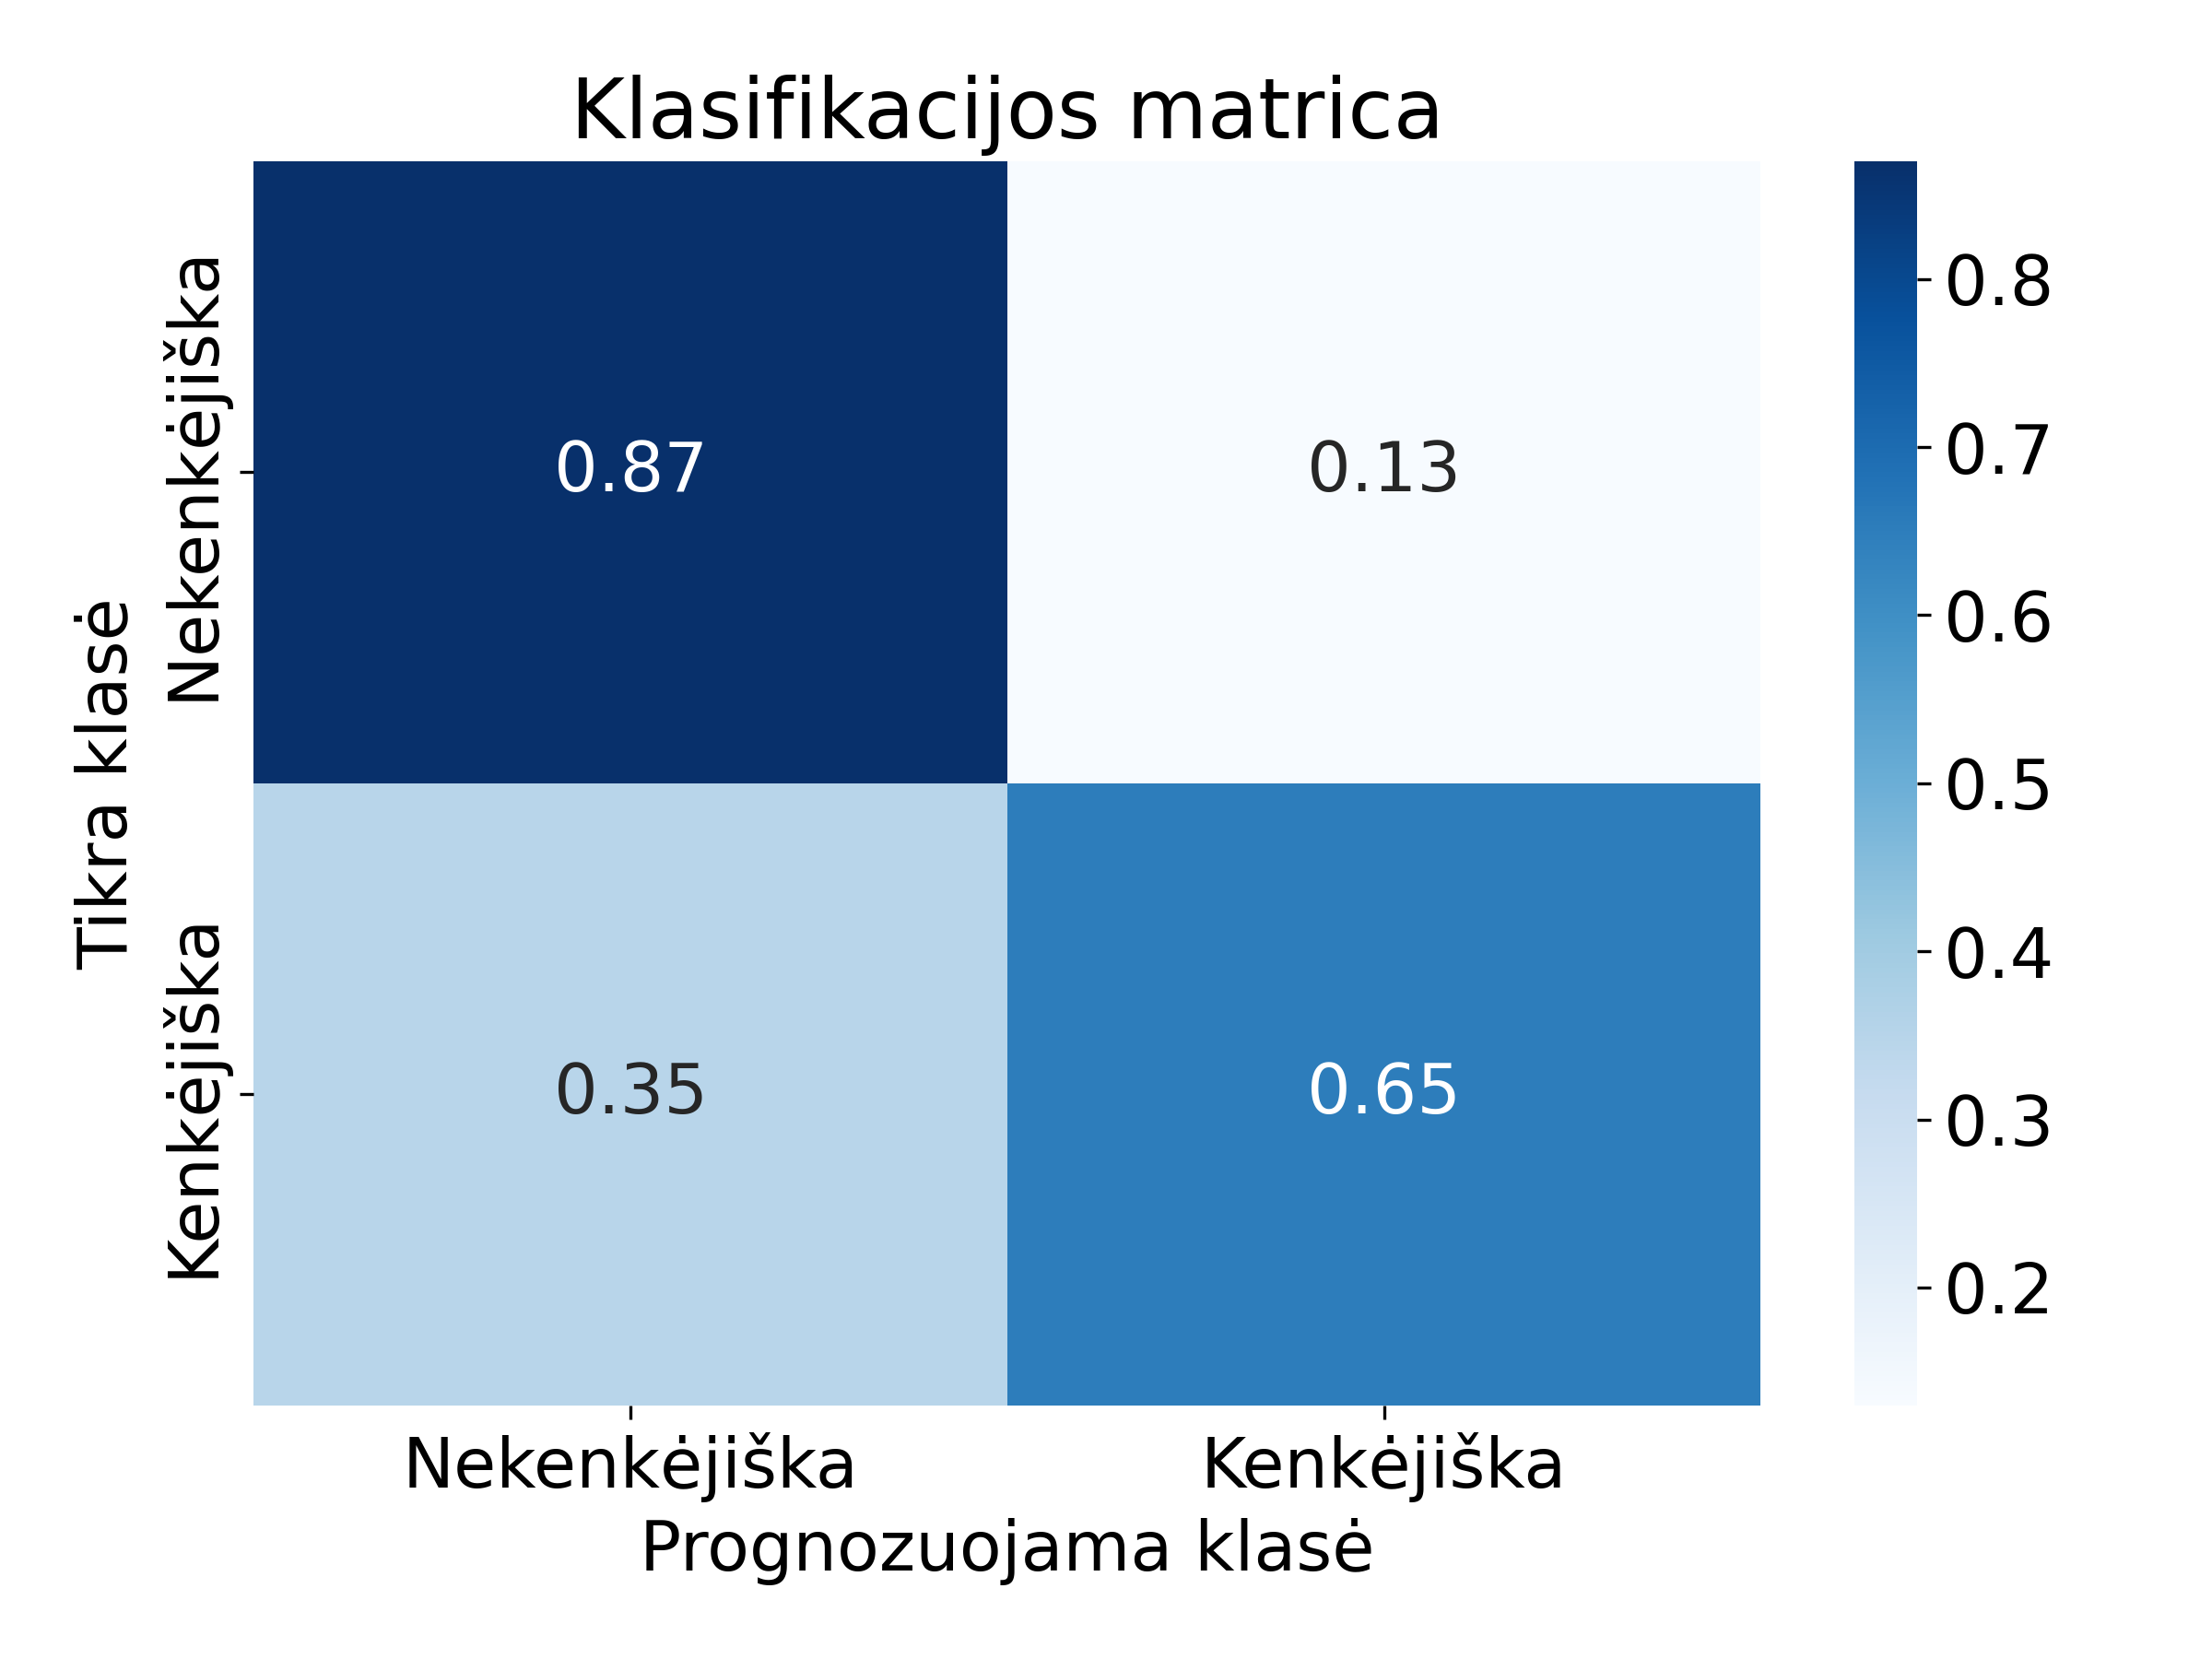
\includegraphics[width=0.5\textwidth]{images/mca_2x2.png}
    \caption{Klasifikavimo matrica}
    \label{fig:exp4:confusion}
\end{figure}

\begin{table}[h]
    \caption{\gls{mca} transformacijos klasifikatoriaus metrikos}
    \centering
    \exptable[\accMcaEquiv]{tables/mca_2x2.csv}
    \label{tbl:exp4:metrics}
\end{table}